\documentclass{article}
\usepackage{hyperref}
\usepackage[margin=1.5in]{geometry}
\usepackage{pdfpages}
\usepackage{minted}
\usepackage{xcolor}
\usepackage{graphicx}
\usepackage{svg}
\usepackage{amsmath}
\usepackage{clrscode3e}
\usepackage{soul}
\usepackage{color}
\usepackage{graphicx}
\usepackage{lscape}

\graphicspath{ {./images/} }

\definecolor{friendlybg}{HTML}{f0f0f0}
\title{Book}
\author{b.skerritt }
\date{October 2019}

\AtBeginEnvironment{minted}{%
  \renewcommand{\fcolorbox}[4][]{#4}}

\addtolength{\parskip}{\baselineskip}

\newcommand{\code}[1]{\texttt{#1}}

\definecolor{bg}{rgb}{0.9, 0.9, 0.9}
\definecolor{monokaibg}{HTML}{272822}
\begin{document}
\pagenumbering{gobble}
\raggedright
\includepdf{algorithmic.pdf}
\newpage
\section{Contributors}
Many thanks to Asmentis, Andreasvirkus for contributing to the book.

If you'd like your name here, contribute to the book on GitHub (typos get your name here too, make an issue).
\tableofcontents
\newpage
\pagenumbering{arabic}
\setcounter{page}{1}
\section{Preface}
Welcome! This book will teach you everything you need to know about algorithmic design paradigms! Using this knowledge will let you design killer algorithms! 

\subsection{Greedy vs Divide and Conquer vs Dynamic Programming}
You may be wondering what the differences are. Fear not! I've created this nifty table for you.
\includegraphics[width=\textwidth,height=\textheight,keepaspectratio]{images/vsdivide.png}
\newpage

\section{Greedy Algorithms}
We start our journey with the simplest of all algorithmic design paradigms. \textbf{Greedy algorithms}.

Greedy algorithms aim to make the optimal choice at that given moment. Each step it chooses the optimal choice, without knowing the future. It attempts to find the globally optimal way to solve the entire problem using this method.

\begin{quote}
    At that exact moment in time, what is the optimal choice to make?
\end{quote}

Greedy algorithms are greedy. They do not look into the future to decide the global optimal solution. They are only concerned with the optimal solution locally. This means that the overall optimal solution may differ from the solution the algorithm chooses.

They never look backwards at what they've done to see if they could optimise globally. This is the main difference between Greedy and Dynamic Programming (discussed later).

To be extra clear, one of the most Googled questions about greedy algorithms is:

\begin{quote}
    "What problem-solving strategies don't guarantee solutions but make efficient use of time?"
\end{quote}

The answer is "Greedy algorithms". They don't guarantee solutions, but are very time efficient. However, in the next section we'll learn that sometimes Greedy solutions give us the optimal solutions.
\newpage
\subsection{What Are Greedy Algorithms Used For?}
Greedy algorithms are quick. A lot faster than the two other alternatives (Divide and Conquer, and Dynamic Programming). They're used because they're fast.

Sometimes, Greedy algorithms give the global optimal solution everytime. Some of these algorithms are:
\begin{itemize}
    \item Dijkstra's Algorithm
    \item Kruskal's Algorithm
    \item Prim's Algorithm
    \item Huffman Trees
\end{itemize}

These algorithms are Greedy, and their Greedy solution gives the optimal solution.
We're going to explore greedy algorithms using examples, and learning how it all works.
\newpage
\subsection{How Do I Create a Greedy Algorithm?}
Your algorithm needs to follow this property:
\begin{quote}
    At that exact moment in time, what is the optimal choice to make?
\end{quote}
And that's it. There isn't much to it. Greedy algorithms are easier to code than Divide and Conquer or Dynamic Programming.
\newpage
\subsection{Counting Change Using Greedy}
Imagine you're a vending machine. Someone gives you £1 and buys a drink for £0.70p. There's no 30p coin in pound sterling, how do you calculate how much change to return?
For reference, this is the denomination of each coin in the UK:

$$1p, 2p, 5p, 10p, 20p, 50p, \pounds 1$$

The greedy algorithm starts from the highest denomination and works backwards. Our algorithm starts at £1. £1 is more than 30p, so it can't use it. It does this for 50p. It reaches 20p. 20p < 30p, so it takes 1 20p.

The algorithm needs to return change of 10p. It tries 20p again, but 20p > 10p. It next goes to 10p. It chooses 1 10p, and now our return is 0 we stop the algorithm.

We return 1x20p and 1x10p.

This algorithm works well in real life. Let's use another example, this time we have the denomination next to how many of that coin is in the machine, 

\begin{minted}[
    style=monokai,
    bgcolor=monokaibg
]{python}
(denomination, how many)
\end{minted}
$$(1p, 10), (2p, 3), (5p, 1), (10p, 0), (20p, 1p), (50p, 19p), (100p, 16)$$

The algorithm is asked to return change of 30p again. 100p (£1) is no. Same for 50. 20p, we can do that. We pick 1x 20p. We now need to return 10p. 20p has run out, so we move down 1.

10p has run out, so we move down 1.

We have 5p, so we choose 1x5p. We now need to return 5p. 5p has run out, so we move down one.
We choose 1 2p coin. We now need to return 3p. We choose another 2p coin. We now need to return 1p. We move down one.

We choose 1x 1p coin. 

Our algorithm selected these coins to return as change:

\begin{minted}[
    style=monokai,
    bgcolor=monokaibg
]{python}
# (value, how many we return as change)
(10, 1)
(5, 1)
(2, 2)
(1, 1)
\end{minted}
 
 Let's code something. First, we need to define the problem. We'll start with the denominations.
 
 \begin{minted}[
    style=monokai,
    bgcolor=monokaibg
]{python}
denominations = [1, 2, 5, 10, 20, 50, 100]
# 100p is £1
\end{minted}
 
 Now onto the core function. Given \code{denomination} and an amount to give change, we want to return a list of how many times that coin was returned. 
 
 If our \code{denominations} list is as above, \code{[6, 3, 0, 0, 0, 0, 0]} represents taking 6 1p coins and 3 2p coins, but 0 of all other coins.
 
 \begin{minted}[
    style=monokai,
    bgcolor=monokaibg
]{python}
denominations = [1, 2, 5, 10, 20, 50, 100]
# 100p is £1

def returnChange(change, denominations):
	toGiveBack = [0] * len(denominations)
	for pos, coin in reversed(list(enumerate(denominations))):

\end{minted}
 We create a list, the size of denominations long and fill it with 0's. 
 
We want to loop backwards, from largest to smallest. \code{Reversed(x)} reverses x and lets us loop backwards. Enumerate means "for loop through this list, but keep the position in another variable". In our example when we start the loop. \code{coin = 100} and \code{pos = 6}.

Our next step is choosing a coin for as long as we can use that coin. If we need to give change = 40 we want our algorithm to choose 20, then 20 again until it can no longer use 20. We do this using a for loop. 
 \begin{minted}[
    style=monokai,
    bgcolor=monokaibg
]{python}
denominations = [1, 2, 5, 10, 20, 50, 100]
# 100p is £1

def returnChange(change, denominations):
	# makes a list size of length denominations filled with 0's
	toGiveBack = [0] * len(denominations)

	# goes backwards through denominations list
	# and also keeps track of the counter, pos.
	for pos, coin in enumerate(reversed(denominations)):
		# while we can still use coin, use it until we can't
		while coin <= change:

\end{minted}
While the coin can still fit into change, add that coin to our return list, toGiveBack and remove it from change.

 \begin{minted}[
    style=monokai,
    bgcolor=monokaibg
]{python}
denominations = [1, 2, 5, 10, 20, 50, 100]
# 100p is £1

def returnChange(change, denominations):
	# makes a list size of length denominations filled with 0
	toGiveBack = [0] * len(denominations)

	# goes backwards through denominations list
	# and also keeps track of the counter, pos.
	for pos, coin in enumerate(reversed(denominations)):
		# while we can still use coin, use it until we can't
		while coin <= change:
			change = change - coin
			toGiveBack[pos] += 1
	return(toGiveBack)
			
print(returnChange(30, denominations))
# returns [0, 0, 0, 1, 1, 0, 0]
# 1x 10p, 1x 20p
\end{minted}
The runtime of this algorithm is dominated by the 2 loops, thus it is $O(n^2)$.
\newpage
\subsection{Is Greedy Optimal? Does Greedy Always Work?}
It is optimal locally, but sometimes it isn't optimal globally. In the change giving algorithm, we can force a point at which it isn't optimal globally. 
The algorithm for doing this is:
\begin{itemize}
    \item Pick 3 denominations of coins. 1p, x, and less than 2x but more than x.
\end{itemize}

We'll pick 1, 15, 25.
\begin{itemize}
    \item Ask for change of 2 * second denomination (15)
\end{itemize}

We'll ask for change of 30. Now, let's see what our Greedy algorithm does.
 \begin{minted}[
    style=monokai,
    bgcolor=monokaibg
]{python}
[5, 0, 1]
\end{minted}
It choses 1x 25p, and 5x 1p. The optimal solution is 2x 15p. 

Our Greedy algorithm failed because it didn't look at 15p. It looked at 25p and thought "yup, that fits. Let's take it."

It then looked at 15p and thought "that doesn't fit, let's move on".

This is an example of where Greedy Algorithms fail.

To get around this, you would either have to create currency where this doesn't work or to brute-force the solution. Or use Dynamic Programming.
\newpage
\subsection{Dijkstra's Algorithm}
Dijkstra's algorithm finds the shortest path from a node to every other node in the graph. In our example, we'll be using a weighted directed graph. Each edge has a direction, and each edge has a weight.

Dijkstra's algorithm has many uses. It can be very useful within road networks where you need to find the fastest route to a place. We also use the algorithm for:
\begin{itemize}
    \item IP Routing
    \item A* Algorithm
    \item Telephone networks
\end{itemize}

The algorithm follows these rules:
\begin{enumerate}
    \item Every time we want to visit a new node, we will choose the node with the smallest known distance.
    \item Once we've moved to the node, we check each of its neighbouring nodes. We calculate the distance from the neighbouring nodes to the root nodes by summing the cost of the edges that lead to that new node.
    \item If the distance to a node is less than a known distance, we'll update the shortest distance.
\end{enumerate}
\includegraphics{Blank-Diagram-33-.png}
Our first step is to pick the starting node. Let's choose A. All the distances start at infinity, as we don't know their distance until we reach a node that knows the distance.
\includegraphics{Blank-Diagram-35-.png}
We mark off A on our unvisited nodes list. The distance from A to A is 0. The distance from A to B is 4. The distance from A to C is 2. We updated our distance listing on the right-hand side.

We pick the smallest edge where the vertex hasn't been chosen. The smallest edge is A -> C, and we haven't chosen C yet. We visit C.

Notice how we're picking the smallest distance from our current node to a node we haven't visited yet. We're being greedy. Here, the greedy method is the global optimal solution.

\includegraphics{Blank-Diagram-36-.png}

We can get to B from C. We now need to pick a minimum. $min(4, 2 + 1) = 3$.

\includegraphics{images/Blank-Diagram-37-.png}
Since A -> C -> B is smaller than A -> B, we update B with this information. We then add in the distances from the other nodes we can now reach.

\includegraphics{Blank-Diagram-40-.png}
Our next smallest vertex with a node we haven't visited yet is B, with 3. We visit B.
\includegraphics{Blank-Diagram-41-.png}
We do the same for B. Then we pick the smallest vertex we haven't visited yet, D.
\includegraphics{Blank-Diagram-42-.png}
We don't update any of the distances this time. Our last node is then E.
\includegraphics[]{Blank-Diagram-43-.png}
There are no updates again. To find the shortest path from A to the other nodes, we walk back through our graph. 

We pick A first, C second, B third. If you need to create the shortest path from A to every other node as a graph, you can run this algorithm using a table on the right-hand side. 
\newpage

\begin{table}[]
\centering
\caption{Dijkstra's Table}
\label{tab:my-table}
\begin{tabular}{|l|l|l|}
\hline
\textbf{Node} & \textbf{Distance from A} & \textbf{Previous Node} \\ \hline
A & 0 & N/A \\ \hline
B & 3 & C \\ \hline
C & 2 & A \\ \hline
D & 5 & B \\ \hline
E & 6 & B \\ \hline
\end{tabular}
\end{table}

Using this table it is easy to draw out the shortest distance from A to every other node in the graph.

\includegraphics{Blank-Diagram-44-.png}
\newpage
\subsection{Minimum Spanning Trees Using Prim's Algorithm}
Prim's algorithm is a greedy algorithm that finds a minimum spanning tree for a weighted undirected graph. It finds the optimal route from every node to every other node in the tree.

With a small change to Dijkstra's algorithm, we can build a new algorithm - Prim's algorithm!

We informally describe the algorithm as:

\begin{enumerate}
    \item Create a new tree with a single vertex (chosen randomly)
    \item Of all the edges not yet in the new tree, find the minimum weighted edge and transfer it to the new tree
    \item Repeat step 2 until all vertices are in the tree
\end{enumerate}
\includegraphics[width=\textwidth,height=\textheight,keepaspectratio]{1.png}
We have this graph. 

Our next step is to pick an arbitrary node. 
\includegraphics[width=\textwidth,height=\textheight,keepaspectratio]{2.png}

We pick the node A. We then examine all the edges connecting A to other vertices. Prim's algorithm is greedy. That means \textbf{it picks the shortest edge that connects to an unvisited vertex.}

In our example, it picks B.

\includegraphics[width=\textwidth,height=\textheight,keepaspectratio]{3.png}

We now look at all nodes reachable from A and B. This is the distinction between Dijkstra's and Prim's. With Dijkstra's, we're looking for a path from 1 node to a certain other node (nodes that have not been visited). With Prim's, we want the minimum spanning tree. 

We have 3 edges with equal weights of 3. We pick 1 randomly.

\includegraphics[width=\textwidth,height=\textheight,keepaspectratio]{4.png}

It is helpful to highlight our graph as we go along, because it makes it easier to create the minimum spanning tree.

\includegraphics[width=\textwidth,height=\textheight,keepaspectratio]{5.png}

Now we look at all edges of A, B, and C. The shortest edge is C > E with a weight of 1.

\includegraphics[width=\textwidth,height=\textheight,keepaspectratio]{6.png}

And we repeat:

\includegraphics[width=\textwidth,height=\textheight,keepaspectratio]{images/withD.png}

The edge $B > E$ with a weight of 3 is the smallest edge. However, both vertices are always in our \code{VISITED} list. Meaning we do not pick this edge. We instead choose $C > F$, as we have not visited 

\includegraphics[width=\textwidth,height=\textheight,keepaspectratio]{withD2.png}
The only node left is G, so let's visit it.

\includegraphics[width=\textwidth,height=\textheight,keepaspectratio]{withD3.png}

Note that if the edge weights are distinct, the minimum spanning tree is unique.

\includegraphics[width=\textwidth,height=\textheight,keepaspectratio]{10.png}

We can add the edge weights to get the minimum spanning tree's total edge weight:
$$2 + 3 + 3 + 1 + 6 + 9 = 24$$
\newpage
\subsection{Fractional Knapsack Problem Using Greedy Algorithm}
Imagine you are a thief. You break into the house of Judy Holliday - 1951 Oscar winner for Best Actress. Judy is a hoarder of gems. Judy's house is lined to the brim with gems.

You brought with you a bag - a knapsack if you will. This bag has a weight of 7. You happened to have a listing of  Judy's items, from some insurance paper. The items read as:

\begin{center}
\begin{tabular}{|l|l|l|}
\hline
\centering
\textbf{Name} & \textbf{Value} & \textbf{Weight} \\ \hline
Diamonds      & 16             & 5               \\ \hline
Francium      & 3              & 1               \\ \hline
Sapphire      & 6              & 2               \\ \hline
Emerald       & 2              & 1               \\ \hline
\end{tabular}
\end{center}
The first step to solving the fractional knapsack problem is to calculate $\frac{value}{weight}$ for each item.

\begin{center}
\begin{tabular}{|l|l|l|l|}
\hline
\centering
\textbf{Name} & \textbf{Value} & \textbf{Weight} & \textbf{Value/weight} \\ \hline
Diamonds      & 16             & 5 & 3.2              \\ \hline
Francium      & 3              & 1    & 3           \\ \hline
Sapphire      & 6              & 2       & 3        \\ \hline
Emerald       & 2              & 1       & 2        \\ \hline
\end{tabular}
\end{center}
And now we greedily select the largest ones. To do this, we can sort them according to $\frac{value}{weight}$ in descending order. Luckily for us, they are already sorted. The largest one is 3.2. 


$$knapsack \;value = 16$$
$$knapsack \;total \;weight = 5 \;(out \;of \;7)$$
Then we select Francium (I know it's not a gem, but Judy is a bit strange ;) )
$$knapsack \;value = 19$$
$$knapsack \;total \;weight = 6 \;(out \;of \;7)$$
Now, we add Sapphire. But if we add Sapphire, our total weight will come to 8. 

In the fractional knapsack problem, we can cut items up to take fractions of them. We have a weight of 1 left in the bag. Our sapphire is weight 2. We calculate the ratio of:
$$\frac{weight\;of\;knapsack\;left}{weight\;of\;item}$$
And then multiply this ratio by the value of the item to get how much value of that item we can take.
$$\frac{1}{2} * 6 = 3$$

$$knapsack \;value = 21$$
$$knapsack \;total \;weight = 7 \;(out \;of \;7)$$

The greedy algorithm can optimally solve the fractional knapsack problem, but it cannot optimally solve the {0, 1} knapsack problem. In this problem instead of taking a fraction of an item, you either take it {1} or you don't {0}. To solve this, you need to use Dynamic Programming (discussed later).

The runtime for this algorithm is O(n log n). Calculating $\frac{value}{weight}$ is O(1). Our main step is sorting from largest $\frac{value}{weight}$, which takes O(n log n) time.
\newpage
\section{Divide and Conquer Algorithms}
\subsection{Introduction}
Often I'll hear about how you can optimise a for loop to be faster or how switch statements are faster than if statements. Most computers have over 1 core, with the ability to support multiple threads. Before worrying about optimising for loops or if statements try to attack your problem from a different angle.

Divide and Conquer is one way to attack a problem from a different angle. Don't worry if you have zero experience or knowledge on the topic. This article is designed to be read by someone with very little programming knowledge.
\newpage
\subsection{What Is Divide and Conquer?}
Divide and conquer is where you divide a large problem up into many smaller, much easier to solve problems. The rather small example below illustrates this.
\begin{center}
\includegraphics[]{a.png}
\end{center}

We take the equation $3 + 6 + 2 + 4$ and cut it down into the smallest set of equations, which is [3 + 6, 2 + 4]. It could also be [2 + 3, 4 + 6]. The order doesn't matter, as long as we turn this one long equation into many smaller equations. 

Let’s say we have 8 numbers:
$$4 + 6 + 3 + 2 + 8 + 7 + 5 + 1$$
We want to add them all together. We first divide the problem into 8 equal sub-problems. We do this by breaking the addition up into individual numbers.
$$4 \;6 \;3 \;2 \;8 \;7 \;5 \;1$$
We then add 2 numbers at a time.
\begin{center}
\includegraphics[width=\textwidth,height=\textheight,keepaspectratio]{b.png}
\end{center}
Then 4 numbers into 8 numbers which is our resultant.
\begin{center}
\includegraphics[width=\textwidth,height=\textheight,keepaspectratio]{c.png}
\end{center}
Why do we break it down to individual numbers at stage 1? Why don't we just start from stage 2? Because while this list of numbers is even if the list was odd you would need to break it down to individual numbers to better handle it.

A divide and conquer algorithm tries to break a problem down into as many little chunks as possible since it is easier to solve with little chunks. It does this with recursion.

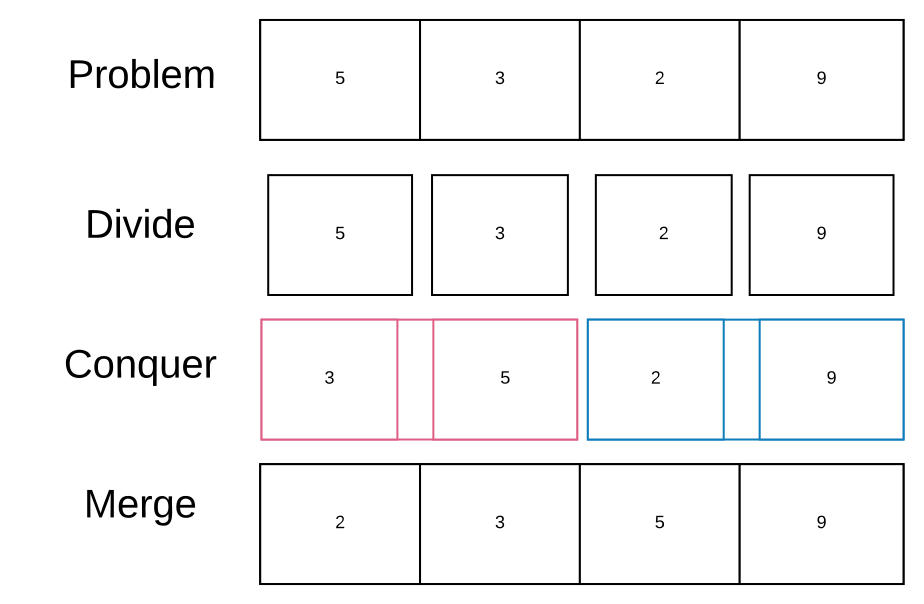
\includegraphics[width=\textwidth,height=\textheight,keepaspectratio]{d.png}

\newpage
\subsection{Recursion}
Before we get into the rest of the article, let's learn about recursion first.

Recursion is when a function calls itself. It's a hard concept to understand if you've never heard of it before.
\includegraphics[width=\textwidth,height=\textheight,keepaspectratio]{e.png}
We open up the bigger one, and inside is a slightly smaller one. Inside that one is another slightly small doll. Let's say, inside the last doll is a key. But we do not know how many dolls there are. How do we write a function that opens up the dolls until we find a key?

We could use a while loop, but recursion is preferred here.
\includegraphics[width=\textwidth,height=\textheight,keepaspectratio]{f.png}
To program this, we can write:
\begin{minted}[
    style=monokai,
    bgcolor=monokaibg
]{python}
def getKey(doll):
	item = doll.open()
    if item == key:
    	return key
	else:
    	return getKey(item)
getKey(doll)
\end{minted}

The function repeatedly calls itself until it finds a key, at which point it stops. The finding key point is called a break case or exit condition.

We always add a break case to a recursive function. If we didn't, it'd just be an infinite loop! Never ending. 

Computer scientists love recursion. Because it's so hard for normal people to understand, we have a schadenfreude sensation watching people struggle. Haha just kidding!

We love recursion because it's used in maths all the time. Computer scientists are mathematicians first, coders second. Anything that brings code closer to real-life mathematics is good. 

Not just because some people love maths, but because it makes it easier to implement. Need to calculate the Fibonacci numbers? The maths equation for this is:



$$F(n) = \begin{cases} n, \text{If n = 0 or 1} \\ F(n - 1) + F(n - 2), \; \text{if n \textgreater \; 1} \end{cases}$$

A natural recurrence in our formula! Instead of translating it into loops, we can just calculate it:

\includegraphics[width=\textwidth,height=\textheight,keepaspectratio]{f.png}
To program this, we can write:
\begin{minted}[
    style=monokai,
    bgcolor=monokaibg
]{python}
def F(n):
	if n == 0 or n == 1:
		return n
  	else:
		return F(n-1)+F(n-2)
\end{minted}
This is one of the reasons why functional programming is so cool.

Also, as you'll see throughout this article, recursion reads so much nicer than loops. And hey, maybe you can feel a little happier when your coworker doesn't understand recursion but you do ;) 
\newpage
\subsection{Back to Divide and Conquer}
The technique is, as defined in the famous Introduction to Algorithms by Cormen, Leiserson, Rivest, and Stein, is:
\begin{itemize}
    \item Divide
\end{itemize}
If the problem is small, then solve it directly. Otherwise, divide the problem into smaller subsets of the same problem.
\begin{itemize}
    \item Conquer
\end{itemize}
Conquer the smaller problems by solving them recursively. If the sub-problems are small enough, recursion is not needed and you can solve them directly.
\begin{itemize}
    \item Combine
\end{itemize}
Take the solutions to the sub-problems and merge them into a solution to the original problem.

Let's look at another example, calculating the factorial of a number.
\begin{minted}[
    style=monokai,
    bgcolor=monokaibg
]{python}
n = 6

def recur_factorial(n):
   if n == 1:
       return n
   else:
       return n * recur_factorial(n-1)

print(recur_factorial(n))
\end{minted}
With the code from above, some important things to note. The Divide part is also the recursion part. We divide the problem up at \code{return n * recur\_factorial(n-1)}.

The \code{recur\_factorial(n-1)} part is where we divide the problem up.

The conquer part is the recursion part too, but also the if statement. If the problem is small enough, we solve it directly (by returning n). Else, we perform \code{return n * recur\_factorial(n-1)}.

Combine. We do this with the multiplication symbol. Eventually, we return the factorial of the number. If we didn't have the symbol there, and it was \code{return recur\_factorial(n-1)} it wouldn't combine and it wouldn't output anything similar to the factorial. (It'll output 1, for those interested).

We'll explore how divide and conquer works in some famous algorithms, Merge Sort and the solution to the Towers of Hanoi.

\subsubsection{One last time}
\begin{enumerate}
    \item Divide / Break. Break the problem into smaller sub-problems.
    \item Conquer / Solve. Solves all the sub-problems.
    \item Merge / Combine. Merges all the sub-solutions into one solution.
\end{enumerate}
\newpage
\subsection{Merge Sort}

Merge Sort is a sorting algorithm. The algorithm works as follows:
\begin{itemize}
    \item Divide the sequence of n numbers into 2 halves
    \item Recursively sort the two halves
    \item Merge the two sorted halves into a single sorted sequence
\end{itemize}

\includegraphics[width=\textwidth,height=\textheight,keepaspectratio]{g.png}

In this image, we break down the 8 numbers into separate digits. Just like we did earlier. Once we've done this, we can begin the sorting process.

It compares 51 and 13. Since 13 is smaller, it puts it in the left-hand side. It does this for (10, 64), (34, 5), (32, 21).

\includegraphics[width=\textwidth,height=\textheight,keepaspectratio]{h.png}

It then merges (13, 51) with (10, 64). It knows that 13 is the smallest in the first list, and 10 is the smallest in the right list. 10 is smaller than 13, therefore we don't need to compare 13 to 64. We're comparing and merging two \textbf{sorted} lists.
\includegraphics[width=\textwidth,height=\textheight,keepaspectratio]{i.png}

In recursion we use the term base case to refer to the absolute smallest value we can deal with. With Merge Sort, the base case is 1. That means we split the list up until we get sub-lists of length 1. That's also why we go down all the way to 1 and not 2. If the base case was 2, we would stop at the 2 numbers.

If the length of the list (n) is larger than 1, then we divide the list and each sub-list by 2 until we get sub-lists of size 1. If n = 1, the list is already sorted so we do nothing.

Merge Sort is an example of a divide and conquer algorithm. Let's look at one more algorithm to understand how divide and conquer works.
\newpage
\subsection{Towers of Hanoi}
The Towers of Hanoi is a mathematical problem which compromises 3 pegs and 3 discs. This problem is mostly used to teach recursion, but it has some real-world uses. The number of pegs and discs can change.
\includegraphics[width=\textwidth,height=\textheight,keepaspectratio]{images/frame_0_delay-1s.png}
Each disc is a different size. We want to move all discs to peg C so that the largest is on the bottom, second largest on top of the largest, third largest (smallest) on top of all of them. There are some rules to this game:
\begin{enumerate}
    \item We can only move 1 disc at a time.
    \item A disc cannot be placed on top of other discs that are smaller than it.
\end{enumerate}
We want to use the smallest number of moves possible. If we have 1 disc, we only need to move it once. 2 discs, we need to move it 3 times.

The number of moves is a power of 2 minus 1. Say we have 4 discs, we calculate the minimum number of moves as $2^4 = 16 - 1 = 15$. 

To solve the above example we want to store the smallest disc in a buffer peg (1 move). See below for a gif on solving Tower of Hanoi with 3 pegs and 3 discs.

Let's run through the solution.
\includegraphics[width=\textwidth,height=\textheight,keepaspectratio]{images/frame_1_delay-1s.png}
 \includegraphics[width=\textwidth,height=\textheight,keepaspectratio]{images/frame_2_delay-1s.png}
 \includegraphics[width=\textwidth,height=\textheight,keepaspectratio]{images/frame_3_delay-1s.png}
 \includegraphics[width=\textwidth,height=\textheight,keepaspectratio]{images/frame_4_delay-1s.png}
 \includegraphics[width=\textwidth,height=\textheight,keepaspectratio]{images/frame_5_delay-1s.png}
 \includegraphics[width=\textwidth,height=\textheight,keepaspectratio]{images/frame_6_delay-1s.png}
 \includegraphics[width=\textwidth,height=\textheight,keepaspectratio]{images/frame_7_delay-1s.png}
 Notice how we need to have a buffer to store the discs.
 
 We can generalise this problem. If we have n discs: move n-1 from A to B recursively, move largest from A to C, move n-1 from B to C recursively.
 
 If there is an even number of pieces the first move is always into the middle. If it is odd the first move is always to the other end.
 
 Let's  code the algorithm for ToH, in pseudocode.
 

		\begin{codebox}
\Procname{$\proc{Towers of Hanoi}(A)$}
\li function MoveTower(disk, source, dest, spare): \Do
    \li if disk == 0, then: \Do
    \li move disk from source to dest
    \End
\end{codebox}
We start with a base case, \code{disk == 0}. \code{source} is the peg you're starting at. \code{dest} is the final destination peg. \code{spare} is the spare peg. 
		\begin{codebox}
\Procname{$\proc{Towers of Hanoi}(A)$}
\li function MoveTower(disk, source, dest, spare): \Do
    \li if disk == 0, then: \Do
    \li move disk from source to dest \End
\li ELSE: \Do
\li move disk from source to dest 
\li MoveTower(disk - 1, spare, dest, source) \End
    \End
\end{codebox}
Notice that with step 1 we switch \code{dest} and \code{source}. We do not do this for step 3. 
With recursion, we know 2 things:
\begin{enumerate}
    \item It always has a base case (if it doesn't, how does the algorithm know to end?)
    \item The function calls itself.
\end{enumerate}
The algorithm gets a little confusing with steps 1 and 3. They both call the same function. This is where multi-threading comes in. You can run steps 1 and 3 on different threads - at the same time. 

Since 2 is more than 1, we move it down one more level again. So far you've seen what the divide and conquer technique is. You should understand how it works and what code looks like. Next, let's learn how to define an algorithm to a problem using divide and conquer. This part is the most important. Once you know this, it'll be easier to create divide and conquer algorithms.

\subsection{How to Solve Problems Using Divide and Conquer}
Now we know how divide and conquer algorithms work, we can build up our own solution. In this example, we'll walk through how to build a solution to the Fibonacci numbers.
\subsubsection{Fibonacci Numbers}

The numbers start at 0 and the next number is the current number + the previous number. But by mathematicla definition, the first 2 numbers are 0 and 1.

Let's say we want to find the 5 Fibonacci number. We can do this:
\begin{minted}[
    style=monokai,
    bgcolor=monokaibg
]{python}
# [0, 1]
0 + 1 = 1 
# [0, 1, 1]
1 + 1 = 2 
# [0, 1, 1, 2]
2 + 1 = 3
# [0, 1, 1, 2, 3]

\end{minted}
Now the first thing when designing a divide and conquer algorithm is to design the recurrence. The recurrence always starts with a base case.

We can describe this relation using a recursion. A recurrence is an equation which defines a function in terms of its smaller inputs. Recurrence and recursion sound similar and are similar.

As we saw, our base case is the 2 numbers at the start.
\begin{minted}[
    style=monokai,
    bgcolor=monokaibg
]{python}
def f(n):
	if n == 0 or n == 1:
    	return n
\end{minted}

To calculate the 4th Fibonacci number, we do (4 - 1) + (4 - 2). This means (last number in the sequence) + (the number before the last).  Or in other words:
\begin{quote}
    The next number is the current number + the previous number.
\end{quote}

If our number is not 0 or 1, we want to add the last 2 Fibonacci numbers together.

Let's take a look at our table quickly:
\begin{minted}[
    style=monokai,
    bgcolor=monokaibg
]{python}
# [0, 1]
0 + 1 = 1
# [0, 1, 1]
1 + 1 = 2 
# [0, 1, 1, 2]
2 + 1 = 3 
# [0, 1, 1, 2, 3]
2 + 3 = 5
# [0, 1, 1, 2, 3, 5]
\end{minted}

But what if we don't have this list stored? How do we calculate the 6th number without creating a list at all? Well we know that the 6th number is the 5th number + the 4th number. Okay, what are those? The 5th number is the 4th number + the 3rd number. The 4th number is the 3rd number + the second number. 

We know that the second number is always 1, as we've reached a base case.

 \includegraphics[width=\textwidth,height=\textheight,keepaspectratio]{fib.png}
 
Eventually we break it down to the basecases. Okay, so we know our code calls itself to calculate the Fibonacci numbers of the previous ones:

\begin{minted}[
    style=monokai,
    bgcolor=monokaibg
]{python}
def f(n):
	if n == 0 or n == 1:
    	return n
	else:
    	f(n-1) f(n-2)
\end{minted}

Okay, how do we merge the Fibonacci numbers at the end? As we saw, it is the last number added to the current number.
\begin{minted}[
    style=monokai,
    bgcolor=monokaibg
]{python}
def f(n):
	if n == 0 or n == 1:
    	return n
	else:
    	f(n-1) + f(n-2)
\end{minted}
Now we've seen this, let's turn it into recursion using a recurrence. Luckily for us, it's incredibly easy to go from a recurrence to code or from code to a recurrence, as they are both recurrences!

$$  F(n) = \begin{cases} n, \text{If n = 0 or 1} \\ F(n - 1) + F(n - 2), \; \text{if n > 1} \end{cases}$$

We often calculate the result of a recurrence using an execution tree. We saw this earlier when exploring how to build it in code. For F(6) this looks like:
\includegraphics[width=\textwidth,height=\textheight,keepaspectratio]{fib.png}
n is 4, and n is larger than 0 or 1. So we do f(n-1) + f(n-2). We ignore the addition for now. This results in 2 new nodes, 3 and 2. 3 is larger than 0 or 1 so we do the same. Same for 2. We do this until we get a bunch of nodes which are either 0 or 1. 

We then add all the nodes together. $0 + 1 + 1 + 0 + 1 + 0 + 1 + 0 + 1 + 0 + 0 + 1 = 8$.

\newpage
\subsection{When Should I Use Divide and Conquer?}
When we have a problem that looks similar to a famous divide and conquer algorithm (such as merge sort), it will be useful.

Most of the time, the algorithms we design will be most similar to merge sort. If we have an algorithm that takes a list and does something with each element of the list, it might be able to use divide and conquer. 

For example, working out the largest item of a list. Given a list of words, how many times does the letter "e" appear? 
\newpage
\subsection{Conclusion}
Once you've identified how to break a problem down into many smaller pieces, you can use concurrent programming to execute these pieces at the same time (on different threads) speeding up the whole algorithm. 

Divide and conquer algorithms are one of the fastest and perhaps easiest ways to increase the speed of an algorithm and are useful in everyday programming.

The next step is to explore multi-threading. Choose your programming language of choice and Google, as an example, "Python multi-threading". Figure out how it works and see if you can attack any problems in your own code from this new angle. 
\newpage
\section{Dynamic Programming}
Dynamic programming is breaking down a problem into smaller sub-problems, solving each sub-problem and storing the solutions to each of these sub-problems in an array (or similar data structure) so each sub-problem is only calculated once. 

It is both a mathematical optimisation method and a computer programming method.

Optimisation problems seek the maximum or minimum solution. The general rule is that if you encounter a problem where the initial algorithm is solved in O($2^n$) time, it is better solved using Dynamic Programming.
\newpage
\subsection{Why Is Dynamic Programming Called Dynamic Programming?}
Richard Bellman invented DP in the 1950s. Bellman named it Dynamic Programming because at the time, RAND (his employer), disliked mathematical research and didn't want to fund it. He named it Dynamic Programming to hide the fact he was really doing mathematical research.

Bellman explains the reasoning behind the term Dynamic Programming in his autobiography, Eye of the Hurricane: An Autobiography (1984, page 159). He explains:
\begin{quote}
    "I spent the Fall quarter (of 1950) at RAND. My first task was to find a name for multistage decision processes. An interesting question is, Where did the name, dynamic programming, come from? The 1950s were not good years for mathematical research. We had a very interesting gentleman in Washington named Wilson. He was Secretary of Defense, and he actually had a pathological fear and hatred of the word research. I’m not using the term lightly; I’m using it precisely. His face would suffuse, he would turn red, and he would get violent if people used the term research in his presence. You can imagine how he felt, then, about the term mathematical. The RAND Corporation was employed by the Air Force, and the Air Force had Wilson as its boss, essentially. Hence, I felt I had to do something to shield Wilson and the Air Force from the fact that I was really doing mathematics inside the RAND Corporation. What title, what name, could I choose? In the first place I was interested in planning, in decision making, in thinking. But planning, is not a good word for various reasons. I decided therefore to use the word “programming”. I wanted to get across the idea that this was dynamic, this was multistage, this was time-varying. I thought, let's kill two birds with one stone. Let's take a word that has an absolutely precise meaning, namely dynamic, in the classical physical sense. It also has a very interesting property as an adjective, and that is it's impossible to use the word dynamic in a pejorative sense. Try thinking of some combination that will possibly give it a pejorative meaning. It's impossible. Thus, I thought dynamic programming was a good name. It was something not even a Congressman could object to. So I used it as an umbrella for my activities."
\end{quote}
\newpage
\subsection{What are Sub-Problems?}
Sub-problems are smaller versions of the original problem. Let's see an example. With the equation below:
$$1 + 2 + 3 + 4$$
We can break this down to:
$$1 + 2$$
$$3 + 4$$
Once we solve these two smaller problems, we can add the solutions to these sub-problems to find the solution to the overall problem.

Notice how these sub-problems breaks down the original problem into components that build up the solution. This is a small example but it illustrates the beauty of Dynamic Programming well. If we expand the problem to adding 100's of numbers it becomes clearer why we need Dynamic Programming. Take this example:
$$6 + 5 + 3 + 3 + 2 + 4 + 6 + 5$$
We have $6 + 5$ twice. The first time we see it, we work out $6 + 5$. When we see it the second time we think to ourselves:
\begin{quote}
    "Ah, 6 + 5. I've seen this before. It's 11!"
\end{quote}
In Dynamic Programming we store the solution to the problem so we do not need to recalculate it. By finding the solutions for every single sub-problem, we can tackle the original problem itself.

\textbf{Memoisation} (not memo\textbf{r}isation) is the act of storing a solution.
\newpage
\subsection{What is Memoisation in Dynamic Programming?}
Let's see why storing answers to solutions make sense. We're going to look at a famous problem, Fibonacci sequence. This problem is normally solved in Divide and Conquer. 

There are 3 main parts to divide and conquer:
\begin{enumerate}
    \item Divide the problem into smaller sub-problems of the same type.
    \item Conquer - solve the sub-problems recursively.
    \item Combine - Combine all the sub-problems to create a solution to the original problem.
\end{enumerate}
Dynamic programming has one extra step added to step 2. This is memoisation. 

The Fibonacci sequence is a sequence of numbers. It's the last number + the current number. We start at 1. 
$$1 + 0 = 1$$
$$1 + 1 = 2$$
$$2 + 1 = 3$$
$$3 + 2 = 5$$
$$5 + 3 = 8$$
In Python, this is:
\begin{minted}[
    style=monokai,
    bgcolor=monokaibg
]{python}
def F(n):
  if n == 0 or n == 1:
	return n
  else:
	return F(n-1)+F(n-2)
\end{minted}
Let's calculate F(4). In an execution tree, this looks like:
 \includegraphics[width=\textwidth,height=\textheight,keepaspectratio]{l.png}
 We calculate F(2) twice. On bigger inputs (such as F(10)) the repetition builds up. The purpose of dynamic programming is to not calculate the same thing twice.
 
 Instead of calculating F(2) twice, we store the solution somewhere and only calculate it once.
 
 We'll store the solution in an array. F[2] = 1. Below is some Python code to calculate the Fibonacci sequence using Dynamic Programming.
 \begin{minted}[
    style=monokai,
    bgcolor=monokaibg
]{python}
 def fibonacciVal(n):
	memo[0], memo[1] = 0, 1
	for i in range(2, n+1):
		memo[i] = memo[i-1] + memo[i-2]
	return memo[n]
\end{minted}
\newpage
\subsection{How to Identify Dynamic Programming Problems}
In theory, Dynamic Programming can solve every problem. The question is then:
\begin{quote}
    "When should I solve this problem with dynamic programming?"
\end{quote}
We should use dynamic programming for problems that are between tractable and intractable problems. 

Tractable problems are those that can be solved in polynomial time. That's a fancy way of saying we can solve it in a fast manner. Binary search and sorting are all fast. Intractable problems are those that run in exponential time. They're slow. Intractable problems are those that can only be solved by bruteforcing through every single combination (NP hard).

When we see terms like:
\begin{quote}
    "shortest/longest, minimized/maximized, least/most, fewest/greatest, "biggest/smallest" 
\end{quote}
We know it's an optimisation problem.

Dynamic Programming algorithms proof of correctness is usually self-evident. Other algorithmic strategies are often much harder to prove correct. Thus, more error-prone.

When we see these kinds of terms, the problem may ask for a specific number ( "find the minimum number of edit operations") or it may ask for a result ( "find the longest common subsequence"). The latter type of problem is harder to recognize as a dynamic programming problem. If something sounds like optimisation, Dynamic Programming can solve it.

Imagine we've found a problem that's an optimisation problem, but we're not sure if it can be solved with Dynamic Programming. First, identify what we're optimising for. Once we realize what we're optimising for, we have to decide how easy it is to perform that optimisation. Sometimes, the greedy approach is enough for an optimal solution. 

Dynamic programming takes the brute force approach. It Identifies repeated work, and eliminates repetition. 

Before we even start to plan the problem as a dynamic programming problem, think about what the brute force solution might look like. Are sub steps repeated in the brute-force solution?  If so, we try to imagine the problem as a dynamic programming problem.

Mastering dynamic programming is all about understanding the problem. List all the inputs that can affect the answers. Once we've identified all the inputs and outputs, try to identify whether the problem can be broken into sub-problems. If we can identify sub-problems, we can probably use Dynamic Programming. 

Then, figure out what the recurrence is and solve it. When we're trying to figure out the recurrence, remember that whatever recurrence we write has to help us find the answer. Sometimes the answer will be the result of the recurrence, and sometimes we will have to get the result by looking at a few results from the recurrence.

Dynamic Programming can solve many problems, but that does not mean there isn't a more efficient solution out there. Solving a problem with Dynamic Programming feels like magic, but remember that dynamic programming is merely a clever brute force. Sometimes it pays off well, and sometimes it helps only a little.

\includegraphics[width=\textwidth,height=\textheight,keepaspectratio]{m.png}
\newpage
\subsection{How to Solve Problems using Dynamic Programming}
Now we have an understanding of what Dynamic programming is and how it generally works. Let's look at to create a Dynamic Programming solution to a problem. We're going to explore the process of Dynamic Programming using the Weighted Interval Scheduling Problem.

Pretend you're the owner of a dry cleaner. You have n customers come in and give you clothes to clean. You can only clean one customer's pile of clothes (PoC) at a time. Each pile of clothes, i, must be cleaned at some pre-determined start time $s_i$ and some predetermined finish time $f_i$.

Each pile of clothes has an associated value, $v_i$, based on how important it is to your business. For example, some customers may pay more to have their clothes cleaned faster. Or some may be repeating customers and you want them to be happy.

As the owner of this dry cleaners you must determine the optimal schedule of clothes that maximises the total value of this day. This problem is a re-wording of the Weighted Interval scheduling problem. 

You will now see 4 steps to solving a Dynamic Programming problem. Sometimes, you can skip a step. Sometimes, your problem is already well defined and you don't need to worry about the first few steps.

\subsubsection{Step 1. Write the Problem out}
Grab a piece of paper. Write out:
\begin{itemize}
    \item What is the problem?
    \item What are the sub-problems?
    \item What would the solution roughly look like?
\end{itemize}

In the dry cleaner problem, let's put down into words the sub-problems. What we want to determine is the maximum value schedule for each pile of clothes such that the clothes are sorted by start time.

Why sort by start time? Good question! We want to keep track of processes which are currently running. If we sort by finish time, it doesn't make much sense in our heads. We could have 2 with similar finish times, but different start times. Time moves in a linear fashion, from start to finish. If we have piles of clothes that start at 1 pm, we know to put them on when it reaches 1pm. If we have a pile of clothes that finishes at 3 pm, we might need to have put them on at 12 pm, but it's  1pm now. 

We can find the maximum value schedule for piles $n - 1$ through to n. And then for $n - 2$ through to n. And so on. By finding the solution to every single sub-problem, we can tackle the original problem itself. The maximum value schedule for piles 1 through n. Sub-problems can be used to solve the original problem, since they are smaller versions of the original problem.

With the interval scheduling problem, the only way we can solve it is by brute-forcing all subsets of the problem until we find an optimal one. What we're saying is that instead of brute-forcing one by one, we divide it up. We brute force from $n-1$ through to n. Then we do the same for $n - 2$ through to n. Finally, we have loads of smaller problems, which we can solve dynamically. We want to build the solutions to our sub-problems such that each sub-problem builds on the previous problems.
\newpage
\subsubsection{Step 2. Mathematical Recurrences}
I know, mathematics sucks. If you'll bare with me here you'll find that this isn't that hard. Mathematical recurrences are used to:
\begin{quote}
    Define the running time of a divide and conquer (dynamic programming) technique
\end{quote}
Recurrences are also used to define problems. If it's difficult to turn your sub-problems into maths, then it may be the wrong sub-problem.

There are 2 steps to creating a mathematical recurrence:

\textbf{1: Define the Base Case}

Base cases are the smallest possible denomination of a problem.

When creating a recurrence, ask yourself these questions:
\begin{quote}
    "What decision do I make at step 0?"
\end{quote}
It doesn't have to be 0. The base case is the smallest possible denomination of a problem. We saw this with the Fibonacci sequence. The base was:
\begin{itemize}
    \item If n == 0 or n == 1, return 1
\end{itemize}
It's important to know where the base case lies, so we can create the recurrence. In our problem, we have one decision to make:
\begin{itemize}
    \item Put that pile of clothes on to be washed
\end{itemize}
or
\begin{itemize}
    \item Don’t wash that pile of clothes today
\end{itemize}
If n is 0, that is, if we have 0 PoC then we do nothing. Our base case is:
\begin{quote}
    if n == 0, return 0
\end{quote}

\textbf{2: What Decision Do I Make at Step n?}

Now we know what the base case is, if we're at step n what do we do? For each pile of clothes that is compatible with the schedule so far. Compatible means that the start time is after the finish time of the pile of clothes currently being washed. The algorithm has 2 options:
\begin{itemize}
    \item Wash that pile of clothes
    \item Don't wash that pile of clothes
\end{itemize}
We know what happens at the base case, and what happens else. We now need to find out what information the algorithm needs to go backwards (or forwards).
\begin{quote}
    "If my algorithm is at step i, what information would it need to decide what to do in step i+1?"
\end{quote}
To decide between the two options, the algorithm needs to know the next compatible PoC (pile of clothes). The next compatible PoC for a given pile, p, is the PoC, n, such that $s_n$ (the start time for PoC n) happens after $f_p$ (the finish time for PoC p). The difference between $s_n$ and $f_p$ should be minimised.

In English, imagine we have one washing machine. We put in a pile of clothes at 13:00. Our next pile of clothes starts at 13:01. We can't open the washing machine and put in the one that starts at 13:00. Our next compatible pile of clothes is the one that starts after the finish time of the one currently being washed.
\begin{quote}
    "If my algorithm is at step i, what information did it need to decide what to do in step i-1?"
\end{quote}
The algorithm needs to know about future decisions. The ones made for PoC i through n to decide whether to run or not run PoC i-1. 

Now that we’ve answered these questions, we’ve started to form a  recurring mathematical decision in our mind. If not, that’s also okay, it becomes easier to write recurrences as we get exposed to more problems.
$$  OPT(i) = \begin{cases} 0, \quad \text{If i = 0} \\ max{v_i + OPT(next[i]), OPT(i+1)},  \quad \text{if n > 1} \end{cases}$$
Let's explore in detail what makes this mathematical recurrence. OPT(i) represents the maximum value schedule for PoC i through to n such that PoC is sorted by start times. OPT(i) is our subproblem from earlier.

We start with the base case. All recurrences need somewhere to stop. If we call OPT(0) we'll be returned with 0.
To determine the value of OPT(i), there are two options. We want to take the maximum of these options to meet our goal. Our goal is the maximum value schedule for all piles of clothes. Once we choose the option that gives the maximum result at step i, we memoize its value as OPT(i).

Mathematically, the two options - run or not run PoC i, are represented as:
$$v_i + OPT(next[n])$$
This represents the decision to run PoC i. It adds the value gained from PoC i to OPT(next[n]), where next[n] represents the next compatible pile of clothing following PoC i. When we add these two values together, we get the maximum value schedule from i through to n such that they are sorted by start time if i runs.
Sorted by start time here because next[n] is the one immediately after $v_i$, so by default, they are sorted by start time.
$$OPT(i + 1)$$
If we decide not to run i, our value is then OPT(i + 1). The value is not gained. OPT(i + 1) gives the maximum value schedule for i+1 through to n, such that they are sorted by start times. 
\newpage
\subsubsection{Step 3. Determine the Dimensions of the Memoisation Array and the Direction in Which It Should Be Filled}
The solution to our Dynamic Programming problem is OPT(1). We can write out the solution as the maximum value schedule for PoC 1 through n such that PoC is sorted by start time. This goes hand in hand with "maximum value schedule for PoC i through to n". 

From step 2:
$$OPT(1) = max(v_1 + OPT(next[1]), OPT(2))$$
Going back to our Fibonacci numbers earlier, our Dynamic Programming solution relied on the fact that the Fibonacci numbers for 0 through to n - 1 were already memoised. That is, to find F(5) we already memoised F(0), F(1), F(2), F(3), F(4). We want to do the same thing here.

The problem we have is figuring out how to fill out a memoisation table. In the scheduling problem, we know that OPT(1) relies on the solutions to OPT(2) and OPT(next[1]). PoC 2 and next[1] have start times after PoC 1 due to sorting. We need to fill our memoisation table from OPT(n) to OPT(1).

We can see our array is one dimensional, from 1 to n. But, if we couldn't see that we can work it out another way. The dimensions of the array are equal to the number and size of the variables on which OPT(x) relies. In our algorithm, we have OPT(i) - one variable, i. This means our array will be 1-dimensional and its size will be n, as there are n piles of clothes.

If we know that n = 5, then our memoisation array might look like this:

memo = [0, OPT(1), OPT(2), OPT(3), OPT(4), OPT(5)]

0 is also the base case. memo[0] = 0, per our recurrence from earlier.

\newpage
\subsubsection{Step 4. Coding Our Solution}
When I am coding a Dynamic Programming solution, I like to read the recurrence and try to recreate it. Our first step is to initialise the array to size (n + 1). In Python, we don't need to do this. But you may need to do it if you're using a different language.

Our second step is to set the base case. 

To find the profit with the inclusion of job[i]. we need to find the latest job that doesn’t conflict with job[i].  The idea is to use Binary Search to find the latest non-conflicting job. I've copied the code from here but edited.

First, let's define what a "job" is. As we saw, a job consists of 3 things:
\begin{minted}[
    style=monokai,
    bgcolor=monokaibg
]{python}
# Class to represent a job 
class Job: 
	def __init__(self, start, finish, profit): 
		self.start = start 
		self.finish = finish 
		self.profit = profit 
\end{minted}
Start time, finish time, and the total profit (benefit) of running that job.

The next step we want to program is the schedule.
\begin{minted}[
    style=monokai,
    bgcolor=monokaibg
]{python}
# The main function that returns the maximum possible 
# profit from given array of jobs
def schedule(job): 
	# Sort jobs according to start time 
	job = sorted(job, key = lambda j: j.start) 

	# Create an array to store solutions of subproblems. table[i] 
	# stores the profit for jobs till arr[i] (including arr[i]) 
	n = len(job) 
	table = [0 for _ in range(n)] 

	table[0] = job[0].profit;
\end{minted}
Earlier, we learnt that the table is 1 dimensional. We sort the jobs by start time, create this empty table and set table[0] to be the profit of job[0]. Since we've sorted by start times, the first compatible job is always job[0].

Our next step is to fill in the entries using the recurrence we learnt earlier. To find the next compatible job, we're using Binary Search. In the full code posted later, it'll include this. For now, let's worry about understanding the algorithm.

If the next compatible job returns -1, that means that all jobs before the index, i, conflict with it (so cannot be used).  Inclprof means we're including that item in the maximum value set. We then store it in table[i], so we can use this calculation again later.
\begin{minted}[
    style=monokai,
    bgcolor=monokaibg
]{python}
    # profit from given array of jobs
	# Fill entries in table[] using recursive property 
	for i in range(1, n): 

		# Find profit including the current job 
		inclProf = job[i].profit 
		l = binarySearch(job, i) 
		if (l != -1): 
			inclProf += table[l]; 

		# Store maximum of including and excluding 
		table[i] = max(inclProf, table[i - 1]) 

\end{minted}
Our final step is then to return the profit of all items up to n-1.
\begin{minted}[
    style=monokai,
    bgcolor=monokaibg
]{python}
	return table[n-1] 
\end{minted}
The full code can be seen below:
\begin{minted}[
    style=monokai,
    bgcolor=monokaibg
]{python}
# Python program for weighted job scheduling using Dynamic 
# Programming and Binary Search 

# Class to represent a job 
class Job: 
	def __init__(self, start, finish, profit): 
		self.start = start 
		self.finish = finish 
		self.profit = profit 


# A Binary Search based function to find the latest job 
# (before current job) that doesn't conflict with current 
# job. "index" is index of the current job. This function 
# returns -1 if all jobs before index conflict with it. 
def binarySearch(job, start_index): 
	# https://en.wikipedia.org/wiki/Binary_search_algorithm

	# Initialize 'lo' and 'hi' for Binary Search 
	lo = 0
	hi = start_index - 1

	# Perform binary Search iteratively 
	while lo <= hi: 
		mid = (lo + hi) // 2
		if job[mid].finish <= job[start_index].start: 
			if job[mid + 1].finish <= job[start_index].start: 
				lo = mid + 1
			else: 
				return mid 
		else: 
			hi = mid - 1
	return -1

# The main function that returns the maximum possible 
# profit from given array of jobs 
def schedule(job): 
	# Sort jobs according to start time 
	job = sorted(job, key = lambda j: j.start) 

	# Create an array to store solutions of subproblems. table[i] 
	# stores the profit for jobs till arr[i] (including arr[i]) 
	n = len(job) 
	table = [0 for _ in range(n)] 

	table[0] = job[0].profit; 

	# Fill entries in table[] using recursive property 
	for i in range(1, n): 

		# Find profit including the current job 
		inclProf = job[i].profit 
		l = binarySearch(job, i) 
		if (l != -1): 
			inclProf += table[l]; 

		# Store maximum of including and excluding 
		table[i] = max(inclProf, table[i - 1]) 

	return table[n-1] 

# Driver code to test above function 
job = [Job(1, 2, 50), Job(3, 5, 20), 
	Job(6, 19, 100), Job(2, 100, 200)] 
print("Optimal profit is"), 
print(schedule(job))
\end{minted}
Congrats! We've just written our first dynamic program!  Now that we’ve wet our feet,  let's walk through a different type of dynamic programming problem.
\newpage
\includepdf{cheatsheet.pdf}
\newpage
\subsection{Knapsack Problem}
Imagine you are a criminal. Dastardly smart. You break into Bill Gates’s mansion. Wow, okay!?!? How many rooms is this? His washing machine room is larger than my entire house??? Ok, time to stop getting distracted. You brought a small bag with you. A knapsack - if you will. 

You can only fit so much into it. Let’s give this an arbitrary number. The bag will support weight 15, but no more. What we want to do is maximise how much money we'll make, $b$.

The greedy approach is to pick the item with the highest value which can fit into the bag. Let's try that. We're going to steal Bill Gates's TV. £4000? Nice. But his TV weighs 15. So... We leave with £4000.
\begin{minted}[
    style=monokai,
    bgcolor=monokaibg
]{python}
TV = (4000, 15)
# (value, weight)
\end{minted}
Bill Gates has a lot of watches. Let's say he has 2 watches. Each watch weighs 5 and each one is worth £2250. When we steal both, we get £4500 with a weight of 10.
\begin{minted}[
    style=monokai,
    bgcolor=monokaibg
]{python}
watch1 = (2250, 5)
watch2 = (2250, 5)
watch1 + watch2
# (£4500, 10)
\end{minted}
In the greedy approach, we wouldn't choose these watches first. But to us as humans, it makes sense to go for smaller items which have higher values. The Greedy approach cannot optimally solve the {0,1} Knapsack problem. The {0, 1} means we either take the item whole item {1} or we don't {0}. However, Dynamic programming can optimally solve the {0, 1} knapsack problem.

The simple solution to this problem is to consider all the subsets of all items. For every single combination of Bill Gates's stuff, we calculate the total weight and value of this combination.

Only those with weight less than $W_{max}$ are considered. We then pick the combination which has the highest value. This is a disaster! How long would this take? Bill Gates's would come back home far before you're even 1/3rd of the way there! In Big O, this algorithm takes $O(n^2)$ time.

You can see we already have a rough idea of the solution and what the problem is, without having to write it down in maths!
\newpage
\subsubsection{Maths Behind {0, 1} Knapsack Problem}
Imagine we had a listing of every single thing in Bill Gates's house. We stole it from some insurance papers. Now, think about the future. What is the optimal solution to this problem?

We have a subset, L, which is the optimal solution. L is a subset of S, the set containing all of Bill Gates's stuff.

Let's pick a random item, N. L either contains N or it doesn't. If it doesn't use N, the optimal solution for the problem is the same as ${1, 2, ..., N-1}$. This is assuming that Bill Gates's stuff is sorted by $value / weight$.

Suppose that the optimum of the original problem is not optimum of the sub-problem. if we have sub-optimum of the smaller problem then we have a contradiction - we should have an optimum of the whole problem.

If L contains N, then the optimal solution for the problem is the same as ${1, 2, 3, ..., N-1}$. We know the item is in, so L already contains N. To complete the computation we focus on the remaining items. We find the optimal solution to the remaining items.

But, we now have a new maximum allowed weight of $W_{max} - W_n$. If item N is contained in the solution, the total weight is now the max weight take away item N (which is already in the knapsack).

These are the 2 cases. Either item N is in the optimal solution or it isn't.

If the weight of item N is greater than $W_{max}$, then it cannot be included so case 1 is the only possibility.

To better define this recursive solution, let $S_k = {1, 2, ..., k}$ and $S_0 = \emptyset$

Let B[k, w] be the maximum total benefit obtained using a subset of $S_k$. Having total weight at most w.

Then we define B[0, w] = 0 for each $w \le W_{max}$.

Our desired solution is then B[n, $W_{max}$].

$$  OPT(i) = \begin{cases} B[k - 1, w], \quad \text{If w < }w_k \\ max{B[k-1, w], b_k + B[k - 1, w - w_k]}, \; \quad \text{otherwise} \end{cases}$$

\newpage
\subsubsection{Tabulation of Knapsack Problem}
Okay, pull out some pen and paper. No, really. Things are about to get confusing real fast. This memoisation table is 2-dimensional. We have these items:
\begin{minted}[
    style=monokai,
    bgcolor=monokaibg
]{python}
(1, 1), (3, 4), (4, 5), (5, 7)
\end{minted}
Where the tuples are \code{(weight, value)}.
We have 2 variables, so our array is 2-dimensional. The first dimension is from 0 to 7. Our second dimension is the values. 

And we want a weight of 7 with maximum benefit.
\begin{center}
\begin{tabular}{|l|l|l|l|l|l|l|l|l|}
\hline
                & \textbf{0} & \textbf{1} & \textbf{2} & \textbf{3} & \textbf{4} & \textbf{5} & \textbf{6} & \textbf{7} \\ \hline
\textbf{(1, 1)} &            &            &            &            &            &            &            &            \\ \hline
\textbf{(4, 3)} &            &            &            &            &            &            &            &            \\ \hline
\textbf{(5, 4)} &            &            &            &            &            &            &            &            \\ \hline
\textbf{(7, 5)} &            &            &            &            &            &            &            &            \\ \hline
\end{tabular}
\end{center}
The weight is 7. We start counting at 0. We put each tuple on the left-hand side. Ok. Now to fill out the table!
\begin{center}
\begin{tabular}{|l|l|l|l|l|l|l|l|l|}
\hline
                & \textbf{0} & \textbf{1} & \textbf{2} & \textbf{3} & \textbf{4} & \textbf{5} & \textbf{6} & \textbf{7} \\ \hline
\textbf{(1, 1)} & 0          &            &            &            &            &            &            &            \\ \hline
\textbf{(4, 3)} & 0          &            &            &            &            &            &            &            \\ \hline
\textbf{(5, 4)} & 0          &            &            &            &            &            &            &            \\ \hline
\textbf{(7, 5)} & 0          &            &            &            &            &            &            &            \\ \hline
\end{tabular}
\end{center}
The columns are weight. At weight 0, we have a total weight of 0. At weight 1, we have a total weight of 1. Obvious, I know. But this is an important distinction to make which will be useful later on.

When our weight is 0, we can't carry anything no matter what. The total weight of everything at 0 is 0.
\begin{center}
\begin{tabular}{|l|l|l|l|l|l|l|l|l|}
\hline
                & \textbf{0} & \textbf{1} & \textbf{2} & \textbf{3} & \textbf{4} & \textbf{5} & \textbf{6} & \textbf{7} \\ \hline
\textbf{(1, 1)} & 0          &1            &            &            &            &            &            &            \\ \hline
\textbf{(4, 3)} & 0          &            &            &            &            &            &            &            \\ \hline
\textbf{(5, 4)} & 0          &            &            &            &            &            &            &            \\ \hline
\textbf{(7, 5)} & 0          &            &            &            &            &            &            &            \\ \hline
\end{tabular}
\end{center}
If our total weight is 1, the best item we can take is (1, 1). As we go down through this array, we can take more items. At the row for (4, 3) we can either take (1, 1) or (4, 3). But for now, we can only take (1, 1). Our maximum benefit for this row then is 1. 
\begin{center}
\begin{tabular}{|l|l|l|l|l|l|l|l|l|}
\hline
                & \textbf{0} & \textbf{1} & \textbf{2} & \textbf{3} & \textbf{4} & \textbf{5} & \textbf{6} & \textbf{7} \\ \hline
\textbf{(1, 1)} & 0          &1            &1            &1            &1            &1            &1            &1            \\ \hline
\textbf{(4, 3)} & 0          &            &            &            &            &            &            &            \\ \hline
\textbf{(5, 4)} & 0          &            &            &            &            &            &            &            \\ \hline
\textbf{(7, 5)} & 0          &            &            &            &            &            &            &            \\ \hline
\end{tabular}
\end{center}
If our total weight is 2, the best we can do is 1. We only have 1 of each item. We cannot duplicate items. So no matter where we are in row 1, the absolute best we can do is (1, 1).

Let's start using (4, 3) now. If the total weight is 1, but the weight of (4, 3) is 3 we cannot take the item yet until we have a weight of at least 3.
\begin{center}
\begin{tabular}{|l|l|l|l|l|l|l|l|l|}
\hline
                & \textbf{0} & \textbf{1} & \textbf{2} & \textbf{3} & \textbf{4} & \textbf{5} & \textbf{6} & \textbf{7} \\ \hline
\textbf{(1, 1)} & 0          &1            &1            &1            &1            &1            &1            &1            \\ \hline
\textbf{(4, 3)} & 0          &1            &1            &            &            &            &            &            \\ \hline
\textbf{(5, 4)} & 0          &            &            &            &            &            &            &            \\ \hline
\textbf{(7, 5)} & 0          &            &            &            &            &            &            &            \\ \hline
\end{tabular}
\end{center}
Now we have a weight of 3. Let's compare some things. We want to take the max of:
$$MAX(4 + T[0][0], 1)$$
If we're at 2, 3 we can either take the value from the last row or use the item on that row. We go up one row and count back 3 (since the weight of this item is 3).

Actually, the formula is whatever weight is remaining when we minus the weight of the item on that row. The weight of (4, 3) is 3 and we're at weight 3. 3 - 3 = 0. Therefore, we're at T[0][0]. T[previous row's number][current total weight - item weight].
$$MAX(4 + T[0][0], 1)$$

The 1 is because of the previous item. The max here is 4.

\begin{center}
\begin{tabular}{|l|l|l|l|l|l|l|l|l|}
\hline
                & \textbf{0} & \textbf{1} & \textbf{2} & \textbf{3} & \textbf{4} & \textbf{5} & \textbf{6} & \textbf{7} \\ \hline
\textbf{(1, 1)} & 0          &1            &1            &1            &1            &1            &1            &1            \\ \hline
\textbf{(4, 3)} & 0          &1            &1            &4            &            &            &            &            \\ \hline
\textbf{(5, 4)} & 0          &            &            &            &            &            &            &            \\ \hline
\textbf{(7, 5)} & 0          &            &            &            &            &            &            &            \\ \hline
\end{tabular}
\end{center}
$$max(4 + t[0][1], 1)$$
Total weight is 4, item weight is 3. 4 - 3 = 1. Previous row is 0. t[0][1].
\begin{center}
\begin{tabular}{|l|l|l|l|l|l|l|l|l|}
\hline
                & \textbf{0} & \textbf{1} & \textbf{2} & \textbf{3} & \textbf{4} & \textbf{5} & \textbf{6} & \textbf{7} \\ \hline
\textbf{(1, 1)} & 0          &1            &1            &1            &1            &1            &1            &1            \\ \hline
\textbf{(4, 3)} & 0          &1            &1            &4            &5            &            &            &            \\ \hline
\textbf{(5, 4)} & 0          &            &            &            &            &            &            &            \\ \hline
\textbf{(7, 5)} & 0          &            &            &            &            &            &            &            \\ \hline
\end{tabular}
\end{center}
I won't bore you with the rest of this row, as nothing exciting happens. We have 2 items. And we've used both of them to make 5. Since there are no new items, the maximum value is 5. 
\begin{center}
\begin{tabular}{|l|l|l|l|l|l|l|l|l|}
\hline
                & \textbf{0} & \textbf{1} & \textbf{2} & \textbf{3} & \textbf{4} & \textbf{5} & \textbf{6} & \textbf{7} \\ \hline
\textbf{(1, 1)} & 0          &1            &1            &1            &1            &1            &1            &1            \\ \hline
\textbf{(4, 3)} & 0          &1            &1            &4            &5            &5            &  5          &  5          \\ \hline
\textbf{(5, 4)} & 0          &            &            &            &            &            &            &            \\ \hline
\textbf{(7, 5)} & 0          &            &            &            &            &            &            &            \\ \hline
\end{tabular}
\end{center}
Onto our next row:
\begin{center}
\begin{tabular}{|l|l|l|l|l|l|l|l|l|}
\hline
                & \textbf{0} & \textbf{1} & \textbf{2} & \textbf{3} & \textbf{4} & \textbf{5} & \textbf{6} & \textbf{7} \\ \hline
\textbf{(1, 1)} & 0          &1            &1            &1            &1            &1            &1            &1            \\ \hline
\textbf{(4, 3)} & 0          &1            &1            &4            &5            &5            &  5          &  5          \\ \hline
\textbf{(5, 4)} & 0          &1            &1            &4            &            &            &            &            \\ \hline
\textbf{(7, 5)} & 0          &            &            &            &            &            &            &            \\ \hline
\end{tabular}
\end{center}
Here's a little secret. Our tuples are ordered by weight! That means that we can fill in the previous rows of data up to the next weight point. We know that 4 is already the maximum, so we can fill in the rest.. This is where memoisation comes into play! We already have the data, why bother re-calculating it?

We go up one row and head 4 steps back. That gives us:
$$max(4 + T[2][0], 5)$$.
\begin{center}
\begin{tabular}{|l|l|l|l|l|l|l|l|l|}
\hline
                & \textbf{0} & \textbf{1} & \textbf{2} & \textbf{3} & \textbf{4} & \textbf{5} & \textbf{6} & \textbf{7} \\ \hline
\textbf{(1, 1)} & 0          &1            &1            &1            &1            &1            &1            &1            \\ \hline
\textbf{(4, 3)} & 0          &1            &1            &4            &5            &5            &  5          &  5          \\ \hline
\textbf{(5, 4)} & 0          &1            &1            &4            &5            &            &            &            \\ \hline
\textbf{(7, 5)} & 0          &            &            &            &            &            &            &            \\ \hline
\end{tabular}
\end{center}
Now we calculate it for total weight 5. 
$$max(5 + T[2][1], 5) = 6$$
\begin{center}
\begin{tabular}{|l|l|l|l|l|l|l|l|l|}
\hline
                & \textbf{0} & \textbf{1} & \textbf{2} & \textbf{3} & \textbf{4} & \textbf{5} & \textbf{6} & \textbf{7} \\ \hline
\textbf{(1, 1)} & 0          &1            &1            &1            &1            &1            &1            &1            \\ \hline
\textbf{(4, 3)} & 0          &1            &1            &4            &5            &5            &  5          &  5          \\ \hline
\textbf{(5, 4)} & 0          &1            &1            &4            &5            &6            &            &            \\ \hline
\textbf{(7, 5)} & 0          &            &            &            &            &            &            &            \\ \hline
\end{tabular}
\end{center}
We do the same thing again:
$$max(5 + T[2][2], 5) = 6$$
\begin{center}
\begin{tabular}{|l|l|l|l|l|l|l|l|l|}
\hline
                & \textbf{0} & \textbf{1} & \textbf{2} & \textbf{3} & \textbf{4} & \textbf{5} & \textbf{6} & \textbf{7} \\ \hline
\textbf{(1, 1)} & 0          &1            &1            &1            &1            &1            &1            &1            \\ \hline
\textbf{(4, 3)} & 0          &1            &1            &4            &5            &5            &  5          &  5          \\ \hline
\textbf{(5, 4)} & 0          &1            &1            &4            &5            &6            &6            &            \\ \hline
\textbf{(7, 5)} & 0          &            &            &            &            &            &            &            \\ \hline
\end{tabular}
\end{center}
Now we have total weight 7. We choose the max of:
$$max(5 + T[2][3], 5) = max(5 + 4, 5) = 9$$
\begin{center}
\begin{tabular}{|l|l|l|l|l|l|l|l|l|}
\hline
                & \textbf{0} & \textbf{1} & \textbf{2} & \textbf{3} & \textbf{4} & \textbf{5} & \textbf{6} & \textbf{7} \\ \hline
\textbf{(1, 1)} & 0          &1            &1            &1            &1            &1            &1            &1            \\ \hline
\textbf{(4, 3)} & 0          &1            &1            &4            &5            &5            &  5          &  5          \\ \hline
\textbf{(5, 4)} & 0          &1            &1            &4            &5            &6            &6            & 9           \\ \hline
\textbf{(7, 5)} & 0          &            &            &            &            &            &            &            \\ \hline
\end{tabular}
\end{center}
If we had total weight 7 and we had the 3 items (1, 1), (4, 3), (5, 4) the best we can do is 9.

Since our new item starts at weight 5, we can copy from the previous row until we get to weight 5.

\begin{center}
\begin{tabular}{|l|l|l|l|l|l|l|l|l|}
\hline
                & \textbf{0} & \textbf{1} & \textbf{2} & \textbf{3} & \textbf{4} & \textbf{5} & \textbf{6} & \textbf{7} \\ \hline
\textbf{(1, 1)} & 0          &1            &1            &1            &1            &1            &1            &1            \\ \hline
\textbf{(4, 3)} & 0          &1            &1            &4            &5            &5            &  5          &  5          \\ \hline
\textbf{(5, 4)} & 0          &1            &1            &4            &5            &6            &6            & 9           \\ \hline
\textbf{(7, 5)} & 0          & 1           & 1           &   4         &   5         &            &            &            \\ \hline
\end{tabular}
\end{center}
We then do another max.

Total weight - new item's weight. This is $5 - 5 = 0$. We want the previous row at position 0.

$$max(7 + T[3][0], 6)$$

The 6 comes from the best on the previous row for that total weight. 
$$max(7 + 0, 6) = 7$$
\begin{center}
\begin{tabular}{|l|l|l|l|l|l|l|l|l|}
\hline
                & \textbf{0} & \textbf{1} & \textbf{2} & \textbf{3} & \textbf{4} & \textbf{5} & \textbf{6} & \textbf{7} \\ \hline
\textbf{(1, 1)} & 0          &1            &1            &1            &1            &1            &1            &1            \\ \hline
\textbf{(4, 3)} & 0          &1            &1            &4            &5            &5            &  5          &  5          \\ \hline
\textbf{(5, 4)} & 0          &1            &1            &4            &5            &6            &6            & 9           \\ \hline
\textbf{(7, 5)} & 0          & 1           & 1           &   4         &   5         &7            &            &            \\ \hline
\end{tabular}
\end{center}
$$max(7 + T[3][1], 6) = 8$$
\begin{center}
\begin{tabular}{|l|l|l|l|l|l|l|l|l|}
\hline
                & \textbf{0} & \textbf{1} & \textbf{2} & \textbf{3} & \textbf{4} & \textbf{5} & \textbf{6} & \textbf{7} \\ \hline
\textbf{(1, 1)} & 0          &1            &1            &1            &1            &1            &1            &1            \\ \hline
\textbf{(4, 3)} & 0          &1            &1            &4            &5            &5            &  5          &  5          \\ \hline
\textbf{(5, 4)} & 0          &1            &1            &4            &5            &6            &6            & 9           \\ \hline
\textbf{(7, 5)} & 0          & 1           & 1           &   4         &   5         &7            & 8           &            \\ \hline
\end{tabular}
\end{center}
$$max(7+T[3][2], 9) = 9$$
\begin{center}
\begin{tabular}{|l|l|l|l|l|l|l|l|l|}
\hline
                & \textbf{0} & \textbf{1} & \textbf{2} & \textbf{3} & \textbf{4} & \textbf{5} & \textbf{6} & \textbf{7} \\ \hline
\textbf{(1, 1)} & 0          &1            &1            &1            &1            &1            &1            &1            \\ \hline
\textbf{(4, 3)} & 0          &1            &1            &4            &5            &5            &  5          &  5          \\ \hline
\textbf{(5, 4)} & 0          &1            &1            &4            &5            &6            &6            & 9           \\ \hline
\textbf{(7, 5)} & 0          & 1           & 1           &   4         &   5         &7            & 8           &9            \\ \hline
\end{tabular}
\end{center}
9 is the maximum value we can get by picking items from the set of items such that the total weight is $\le 7$.
\newpage
\subsubsection{Finding the Optimal Set for {0, 1} Knapsack Problem Using Dynamic Programming}
Now, what items do we actually pick for the optimal set? We start with this item:
\begin{center}
\begin{tabular}{|l|l|l|l|l|l|l|l|l|}
\hline
                & \textbf{0} & \textbf{1} & \textbf{2} & \textbf{3} & \textbf{4} & \textbf{5} & \textbf{6} & \textbf{7} \\ \hline
\textbf{(1, 1)} & 0          &1            &1            &1            &1            &1            &1            &1            \\ \hline
\textbf{(4, 3)} & 0          &1            &1            &4            &5            &5            &  5          &  5          \\ \hline
\textbf{(5, 4)} & 0          &1            &1            &4            &5            &6            &6            & 9           \\ \hline
\textbf{(7, 5)} & 0          & 1           & 1           &   4         &   5         &7            & 8           &\hl{9}            \\ \hline
\end{tabular}
\end{center}
We want to know where the 9 comes from. It's coming from the top because the number directly above 9 on the 4th row is 9. Since it's coming from the top, the item (7, 5) is not used in the optimal set.

Where does this 9 come from?
\begin{center}
\begin{tabular}{|l|l|l|l|l|l|l|l|l|}
\hline
                & \textbf{0} & \textbf{1} & \textbf{2} & \textbf{3} & \textbf{4} & \textbf{5} & \textbf{6} & \textbf{7} \\ \hline
\textbf{(1, 1)} & 0          &1            &1            &1            &1            &1            &1            &1            \\ \hline
\textbf{(4, 3)} & 0          &1            &1            &4            &5            &5            &  5          &  5          \\ \hline
\textbf{(5, 4)} & 0          &1            &1            &4            &5            &6            &6            & \hl{9}           \\ \hline
\textbf{(7, 5)} & 0          & 1           & 1           &   4         &   5         &7            & 8           &9            \\ \hline
\end{tabular}
\end{center}
This 9 is not coming from the row above it. Item (5, 4) must be in the optimal set.

We now go up one row, and go back 4 steps. 4 steps because the item, (5, 4), has weight 4.
\begin{center}
\begin{tabular}{|l|l|l|l|l|l|l|l|l|}
\hline
                & \textbf{0} & \textbf{1} & \textbf{2} & \textbf{3} & \textbf{4} & \textbf{5} & \textbf{6} & \textbf{7} \\ \hline
\textbf{(1, 1)} & 0          &1            &1            &1            &1            &1            &1            &1            \\ \hline
\textbf{(4, 3)} & 0          &1            &1            &\hl{4}            &5            &5            &  5          &  5          \\ \hline
\textbf{(5, 4)} & 0          &1            &1            &4            &5            &6            &6            & 9           \\ \hline
\textbf{(7, 5)} & 0          & 1           & 1           &   4         &   5         &7            & 8           &9            \\ \hline
\end{tabular}
\end{center}
4 does not come from the row above. The item (4, 3) must be in the optimal set.

The weight of item (4, 3) is 3. We go up and we go back 3 steps and reach:
\begin{center}
\begin{tabular}{|l|l|l|l|l|l|l|l|l|}
\hline
                & \textbf{0} & \textbf{1} & \textbf{2} & \textbf{3} & \textbf{4} & \textbf{5} & \textbf{6} & \textbf{7} \\ \hline
\textbf{(1, 1)} & \hl{0}          &1            &1            &1            &1            &1            &1            &1            \\ \hline
\textbf{(4, 3)} & 0          &1            &1            &4            &5            &5            &  5          &  5          \\ \hline
\textbf{(5, 4)} & 0          &1            &1            &4            &5            &6            &6            & 9           \\ \hline
\textbf{(7, 5)} & 0          & 1           & 1           &   4         &   5         &7            & 8           &9            \\ \hline
\end{tabular}
\end{center}
As soon as we reach a point where the weight is 0, we're done. Our two selected items are (5, 4) and (4, 3). The total weight is 7 and our total benefit is 9. We add the two tuples together to find this out. 

Let's begin coding this. 
\newpage
\subsubsection{Coding {0, 1} Knapsack Problem in Dynamic Programming With Python}
Now we know how it works, and we've derived the recurrence for it - it shouldn't be too hard to code it. If our two-dimensional array is i (row) and j (column) then we have:
\begin{minted}[
    style=monokai,
    bgcolor=monokaibg
]{python}
if j < wt[i]:
\end{minted}
If our weight j is less than the weight of item i (i does not contribute to j) then:
\begin{minted}[
    style=monokai,
    bgcolor=monokaibg
]{python}
if j < wt[i]:
	T[i][j] = T[i - 1][j]
else:
	// weight of i >= j
    T[i][j] = max(val[i] + t[i - 1][j-wt(i), t[i-1][j])
    // previous row, subtracting the weight of the item from the total weight or without including ths item
\end{minted}
This is what the core heart of the program does. I've copied some code from here to help explain this. I'm not going to explain this code much, as there isn't much more to it than what I've already explained.
\begin{minted}[
    style=monokai,
    bgcolor=monokaibg
]{python}
# Returns the maximum value that can be put in a knapsack of 
# capacity W 
def knapSack(W , wt , val , n): 
  
    # Base Case 
    if n == 0 or W == 0: 
        return 0
  
    # If weight of the nth item is more than Knapsack of capacity 
    # W, then this item cannot be included in the optimal solution 
    if (wt[n-1] > W): 
        return knapSack(W , wt , val , n-1) 
  
    # return the maximum of two cases: 
    # (1) nth item included 
    # (2) not included 
    else: 
        return max(val[n-1] + knapSack(W-wt[n-1] , wt , val , n-1), 
                   knapSack(W , wt , val , n-1)) 
  
  
# To test above function 
val = [60, 100, 120] 
wt = [10, 20, 30] 
W = 50
n = len(val) 
print(knapSack(W , wt , val , n))
# output 220
\end{minted}
\newpage
\subsection{Time Complexity of a Dynamic Programming Problem}
Time complexity is calculated in Dynamic Programming as:
$$Number \;of \;unique \;states * time \;taken \;per\; state$$
For our original problem, the Weighted Interval Scheduling Problem, we had n piles of clothes. Each pile of clothes is solved in constant time. The time complexity is:
$$O(n) + O(1) = O(n)$$
With our Knapsack problem, we had n number of items. The table grows depending on the total capacity of the knapsack, our time complexity is:
$$O(nw)$$
Where n is the number of items, and w is the capacity of the knapsack.

I'm going to let you in on a little secret. It's possible to work out the time complexity of an algorithm from its recurrence. You can use something called the Master Theorem to work it out. This is the theorem in a nutshell:
\includegraphics[width=\textwidth,height=\textheight,keepaspectratio]{master.png}
\newpage
\subsection{Dynamic Programming vs Divide and Conquer vs Greedy}
Dynamic Programming and Divide and Conquer are similar. Dynamic Programming is based on Divide and Conquer, except we memoise the results.

But, Greedy is different. It aims to optimise by making the best choice at that moment. Sometimes, this doesn't optimise for the whole problem. Take this question as an example. We have 3 coins:

1p, 15p, 25p

And someone wants us to give a change of 30p. With Greedy, it would select 25, then 5 * 1 for a total of 6 coins. The optimal solution is 2 * 15. Greedy works from largest to smallest. At the point where it was at 25, the best choice would be to pick 25. 

\newpage
\subsection{Tabulation (Bottom-Up) vs Memoisation (Top-Down)}
There are 2 types of dynamic programming. Tabulation and Memoisation. 
\subsubsection{Memoisation (Top-Down)}
We've computed all the subproblems but have no idea what the optimal evaluation order is. We would then perform a recursive call from the root, and hope we get close to the optimal solution or obtain a proof that we will arrive at the optimal solution. Memoisation ensures you never recompute a subproblem because we cache the results, thus duplicate sub-trees are not recomputed. 
\includegraphics[width=\textwidth,height=\textheight,keepaspectratio]{ugly.png}
From our Fibonacci sequence earlier, we start at the root node. The subtree F(2) isn't calculated twice.

This starts at the top of the tree and evaluates the subproblems from the leaves/subtrees back up towards the root. Memoisation is a top-down approach.
\subsubsection{Tabulation (Bottom-Up)}
We've also seen Dynamic Programming being used as a 'table-filling' algorithm. Usually, this table is multidimensional. This is like memoisation, but with one major difference. We have to pick the exact order in which we will do our computations. The knapsack problem we saw, we filled in the table from left to right - top to bottom. We knew the exact order of which to fill the table.

Sometimes the 'table' is not like the tables we've seen. It can be a more complicated structure such as trees. Or specific to the problem domain, such as cities within flying distance on a map.
\subsubsection{Tabulation and Memosation - Advantages and Disadvantages}
Generally speaking, memoisation is easier to code than tabulation. We can write a 'memoriser' wrapper function that automatically does it for us. With tabulation, we have to come up with an ordering.

Memoisation has memory concerns. If we're computing something large such as F($10^8$), each computation will be delayed as we have to place them into the array. And the array will grow in size very quickly. And the array will grow in size very quickly.

Either approach may not be time-optimal if the order we happen (or try to) visit subproblems is not optimal.  If there is more than one way to calculate a subproblem (normally caching would resolve this, but it's theoretically possible that caching might not in some exotic cases). Memoisation will usually add on our time-complexity to our space-complexity. For example with tabulation we have more liberty to throw away calculations, like using tabulation with Fib lets us use O(1) space, but memoisation with Fib uses O(N) stack space).
\newpage
\includegraphics[width=\textwidth,height=\textheight,keepaspectratio]{images/donkey.png}
\newpage
\section{Conclusion}
So we've reached the end of my marvelous mystical tour of algorithmic design paradigms! Huzzah! 

Thank you for reading, it means a lot to me :) Have a nice day!

\end{document}